\chapter{Discussion and Conclusion}
As in the past chapters, the methods used and results produced are discussed step by step based on the three main contributions of this thesis.
\section{Implementation of the FD Solver}
First, anomalies in the implementation of the FD solver are discussed.\\
\\
\textbf{Non-negligibility of Sand Layers}
\\
To reasonably include the experimental data produced by Bierbaum et al. \cite{Bierbaum2022Mar}, the neglect of sand is not possible because of dispersion effects of PFOS into the sand layers. At the lower edge, the outward flow of PFOS is delayed due to the sand layer. This behavior was taken into account by Hydrus (Fig. \ref{fig:disc_hydrus_sand}) as well as in the implemented FD solver and FINN (Fig. \ref{fig:disc_ov_hyd_fd_sand_10d}). 
\begin{figure}
	\centering
	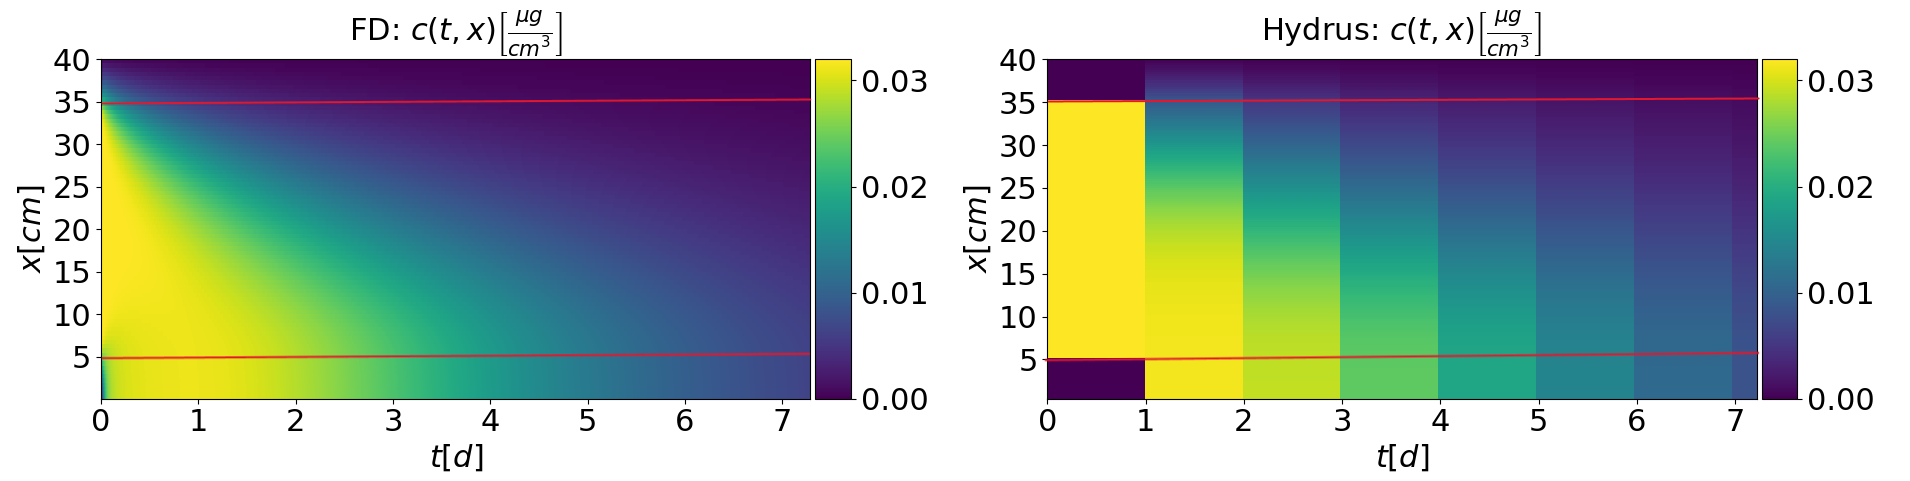
\includegraphics[width=\textwidth]{images/disc_ov_hyd_fd_sand_10d.png}
\caption[Closer look at Hydrus and FD solution]{Closer look at comparison of Hydrus and FD solution with 2 sand layers. Hydrus solution (right), FD solution (left). First 7 days of 200 days total simulation time. Due to Hydrus limitations, data was only tapped at 200 points in time, which results in the rough temporal resolution. Internally, the time discretization of Hydrus is finer. Cells above the upper red line and below the lower red line are the sand layers. Dispersion of PFOS into the upper sand layer can be observed in both solutions.}
\label{fig:disc_ov_hyd_fd_sand_10d}
\end{figure}
\begin{figure}
	\centering
	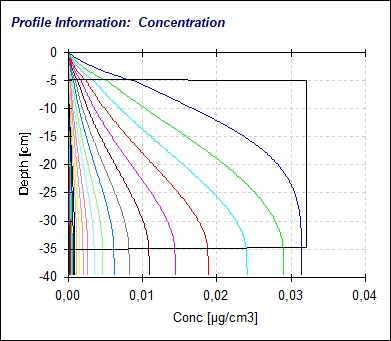
\includegraphics[scale=0.7]{images/hyd_sand_profile.jpg}
\caption[Closer look at the Hydrus solution]{Closer look at the Hydrus solution, using Hydrus visualization tools. Colored are the courses of the dissolved concentration over the contaminated soil length at different times. Regions above and below the horizontal black line, which is the dissolved concentration at $t=0d$, are sand layers. Dispersion of PFOS into the upper sand layer can be observed.}
\label{fig:disc_hydrus_sand}
\end{figure}\\
\\
\textbf{Deviations between FD and Hydrus Solution}
\\
Hydrus can be used to simulate a wide variety of flow and transport processes, which can result in a large number of potential operating errors. Within the scope of this work, the Hydrus settings were extensively investigated, exchanged with the developers in the Hydrus forum and adapted to the parameters of the FD solution, but deviations still occurred.\\
\\
In addition to errors in understanding, the handling of boundary conditions can be a reason for deviations. For example, in the FD solver it was assumed that in the case of no mass transfer between spatial cells, i.e. effective velocity $v = 0$ and molecular diffusion $D=0$, no information exchange takes place across the cells, not even at the edge. Thus, each cell should describe the same process over time.\\
This assumption was tested using Hydrus with identical settings. In particular, the boundary conditions as described in Chapter 2 were adopted: Dirichlet boundary condition at the inlet and Neumann boundary condition at the outlet. It turned out that in Hydrus at the top cell, spatial mass transport occured (Figs. \ref{fig:hyd_zero_transp_c}, \ref{fig:hyd_zero_transp_sk}, corresponding Hydrus file is available on GitHub \cite{Hydrus_BA}). This could be partly due to the fact that the treatment of boundary conditions and spatial discretization is handled differently in FE method compared to FD or FV method. However, the Fortran implementation of Hydrus was not considered further in this work.\\
It could be further investigated how an increased number of spatial discretization steps affects the deviations in order to minimize effects of the different methods in spatial discretization.
\begin{figure}
	\centering
	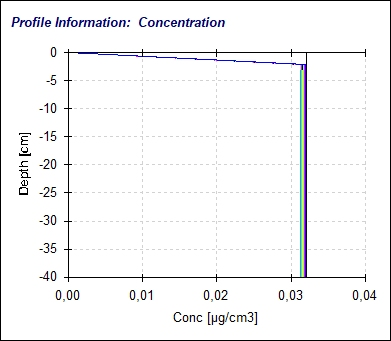
\includegraphics[scale=0.7]{images/ZeroTransport_c.jpg}
\caption[Course of the dissolved concentration in Hydrus]{Dissolved concentration of a substance, simulated in Hydrus with no water flux. Colored: Different observation times.}
\label{fig:hyd_zero_transp_c}
\end{figure}
\begin{figure}
	\centering
	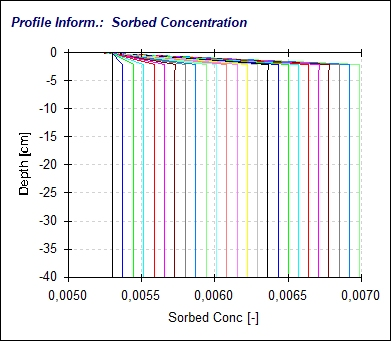
\includegraphics[scale=0.7]{images/ZeroTransport.jpg}
\caption[Course of the kinetically sorbed concentration in Hydrus]{Kin. sorbed concentration with Hydrus settings as in Fig.  \ref{fig:hyd_zero_transp_c}. Colored: Different observation times.}
\label{fig:hyd_zero_transp_sk}
\end{figure}
\\
In addition, Hydrus uses $f=0.9999$ as the fraction between instantaneously and kinetically sorbed concentration in the sand layer, when in fact in the FD solver $f=1.0$ applies, since no sorption occurs.\\
The MSE calculation also leads to small deviations: Due to the time discretization used in the FD method, values of the solution are not present at the exact same times as in the Hydrus solution (Fig. \ref{fig:disc_ov_hyd_fd_sand_10d}).
\section{Embedding of the Transport Equation into the FINN Framework}
Using DNNs to approximate $F$, $G$ and $R$ required many reflections about the architecture of the DNNs, the optimizer, or the loss function to choose, which is a fundamental challenge in Deep Learning. There is no formula with that the perfect number of hidden layers, or number of neurons can be calculated \cite{Stathakis2009Apr}. Also for the choice of activation functions, especially within the DNN, many possibilities are available, which can only be verified empirically and in a time-consuming manner. Of course, heuristics can be used to facilitate the process of the DNN design, which is done for example in DNN puring \cite{Blalock2020Mar}. However, in the present work a very specific DNN was created, which computes unknown functions in a PDE model during time integration, where these heuristics can only be applied to a limited extent. A larger number of used neurons and hidden layers, takes a longer computing time during training, as well as might overfit the training data if training occured for too many epochs, i.e. good training results but bad test results.\\
Batch data sets as random parts of the input data set for the DNN, are commonly used during training to save computational effort when performing optimization. In this work this was also challenging, because for the loss calculation for each time step forward evaluations of the DNNs were needed. In the backward pass, time points and location points used during the integration of the spatially discretized PDE would have to be selected. For this, the torchdiffeq library \cite{torchdiffeq} would have to be expanded. However, the use of no batches can prolong the training enormously, since for each of the $T_{STEPS} \cdot X_{STEPS}$ samples per DNN, corresponding gradients have to be computed. In particular, this process requires a lot of RAM.\\
The unusual usage of the DNNs is followed by the question of how much physical information must be made available to the DNN in order to produce useful results. In this work, the degrees of freedom of the DNN were kept rather low, in contrast to other pure machine learning NNs \cite{Kalchbrenner2016Oct, Karlbauer2019Dec}. To compensate scarce experimental data, in this work FINN was provided all physical information, in solving the PDE. No stencils were learned. Only parameters were optimized or functional relations occuring in the PDE were learned, which were even further constrained with physical information (Loss penalty for negatively learned $c$ or $s_k$, $R \geq 1$, etc.). Also, the separation that each of the functional relations was approximated by its own NN can be considered as a physical information for FINN.\\
So-called Bayesian NNs  \cite{Jospin2022Apr} could provide a way to figure out which of the physical information described above is necessary, leads to underfitting or overfitting, or may be incorrect by quantifying uncertainties of the predicted solution.\\
With PyTorch, it is also possible to move the training and testing of the DNNs to GPU without much additional effort. This leads to a significant time saving in the calculation and makes it easier to adjust the properties of the DNN \cite{Li2016Oct}.
\section{Application of FINN on Experimental Data}
To calculate the initial conditions from the mass balance eq. \ref{eq:mass_cons}, parameters were used which, if necessary, still have to be learned, which is a circular argumentation. However, solving a PDE is not possible without initial conditions, and since the parameters $f$, $k_d$, and $\beta$ according to Bierbaum et al. and run f, described experimental BTCs quite well, they were nevertheless used for the calculation of initial conditions.\\
\\
It has not yet been clarified in the context of this work whether it makes sense to make the learnable functional relations explicitly time-dependent:\\
For the training procedures that based on synthetic data there is only given an implicit time dependancy in the model equations. Nevertheless, this approach was followed for testing purposes with the expectation, that the DNNs are still able to approximate these functions. They should learn a neglect of explicit time dependency.\\
Concerning training based on experimental data we knew that the experimental flow rates changed over the duration of the experiment at each sampling interval because a different pump rate was chosen or the pump tubing wore out \cite{Bierbaum2022Mar}. In order to take these non-negligible fluctuations (Fig. \ref{fig:different_velocities}) and also probably chemical reasons for changes of $F$, $G$ and $R$ explicitly in time into consideration, in the majority of the sessions an explicit time dependency was used. Future work could include a detailed investigation of this topic by for example learning non time-dependent functional relations but approximating the changes of experimental flow rates by another DNN as a function in time.\\
The overestimated $s_k$ at the simulation end, learned in run h could be embedded in the loss function analogously to negatively learned concentrations and be punished.
\begin{figure}
	\centering
	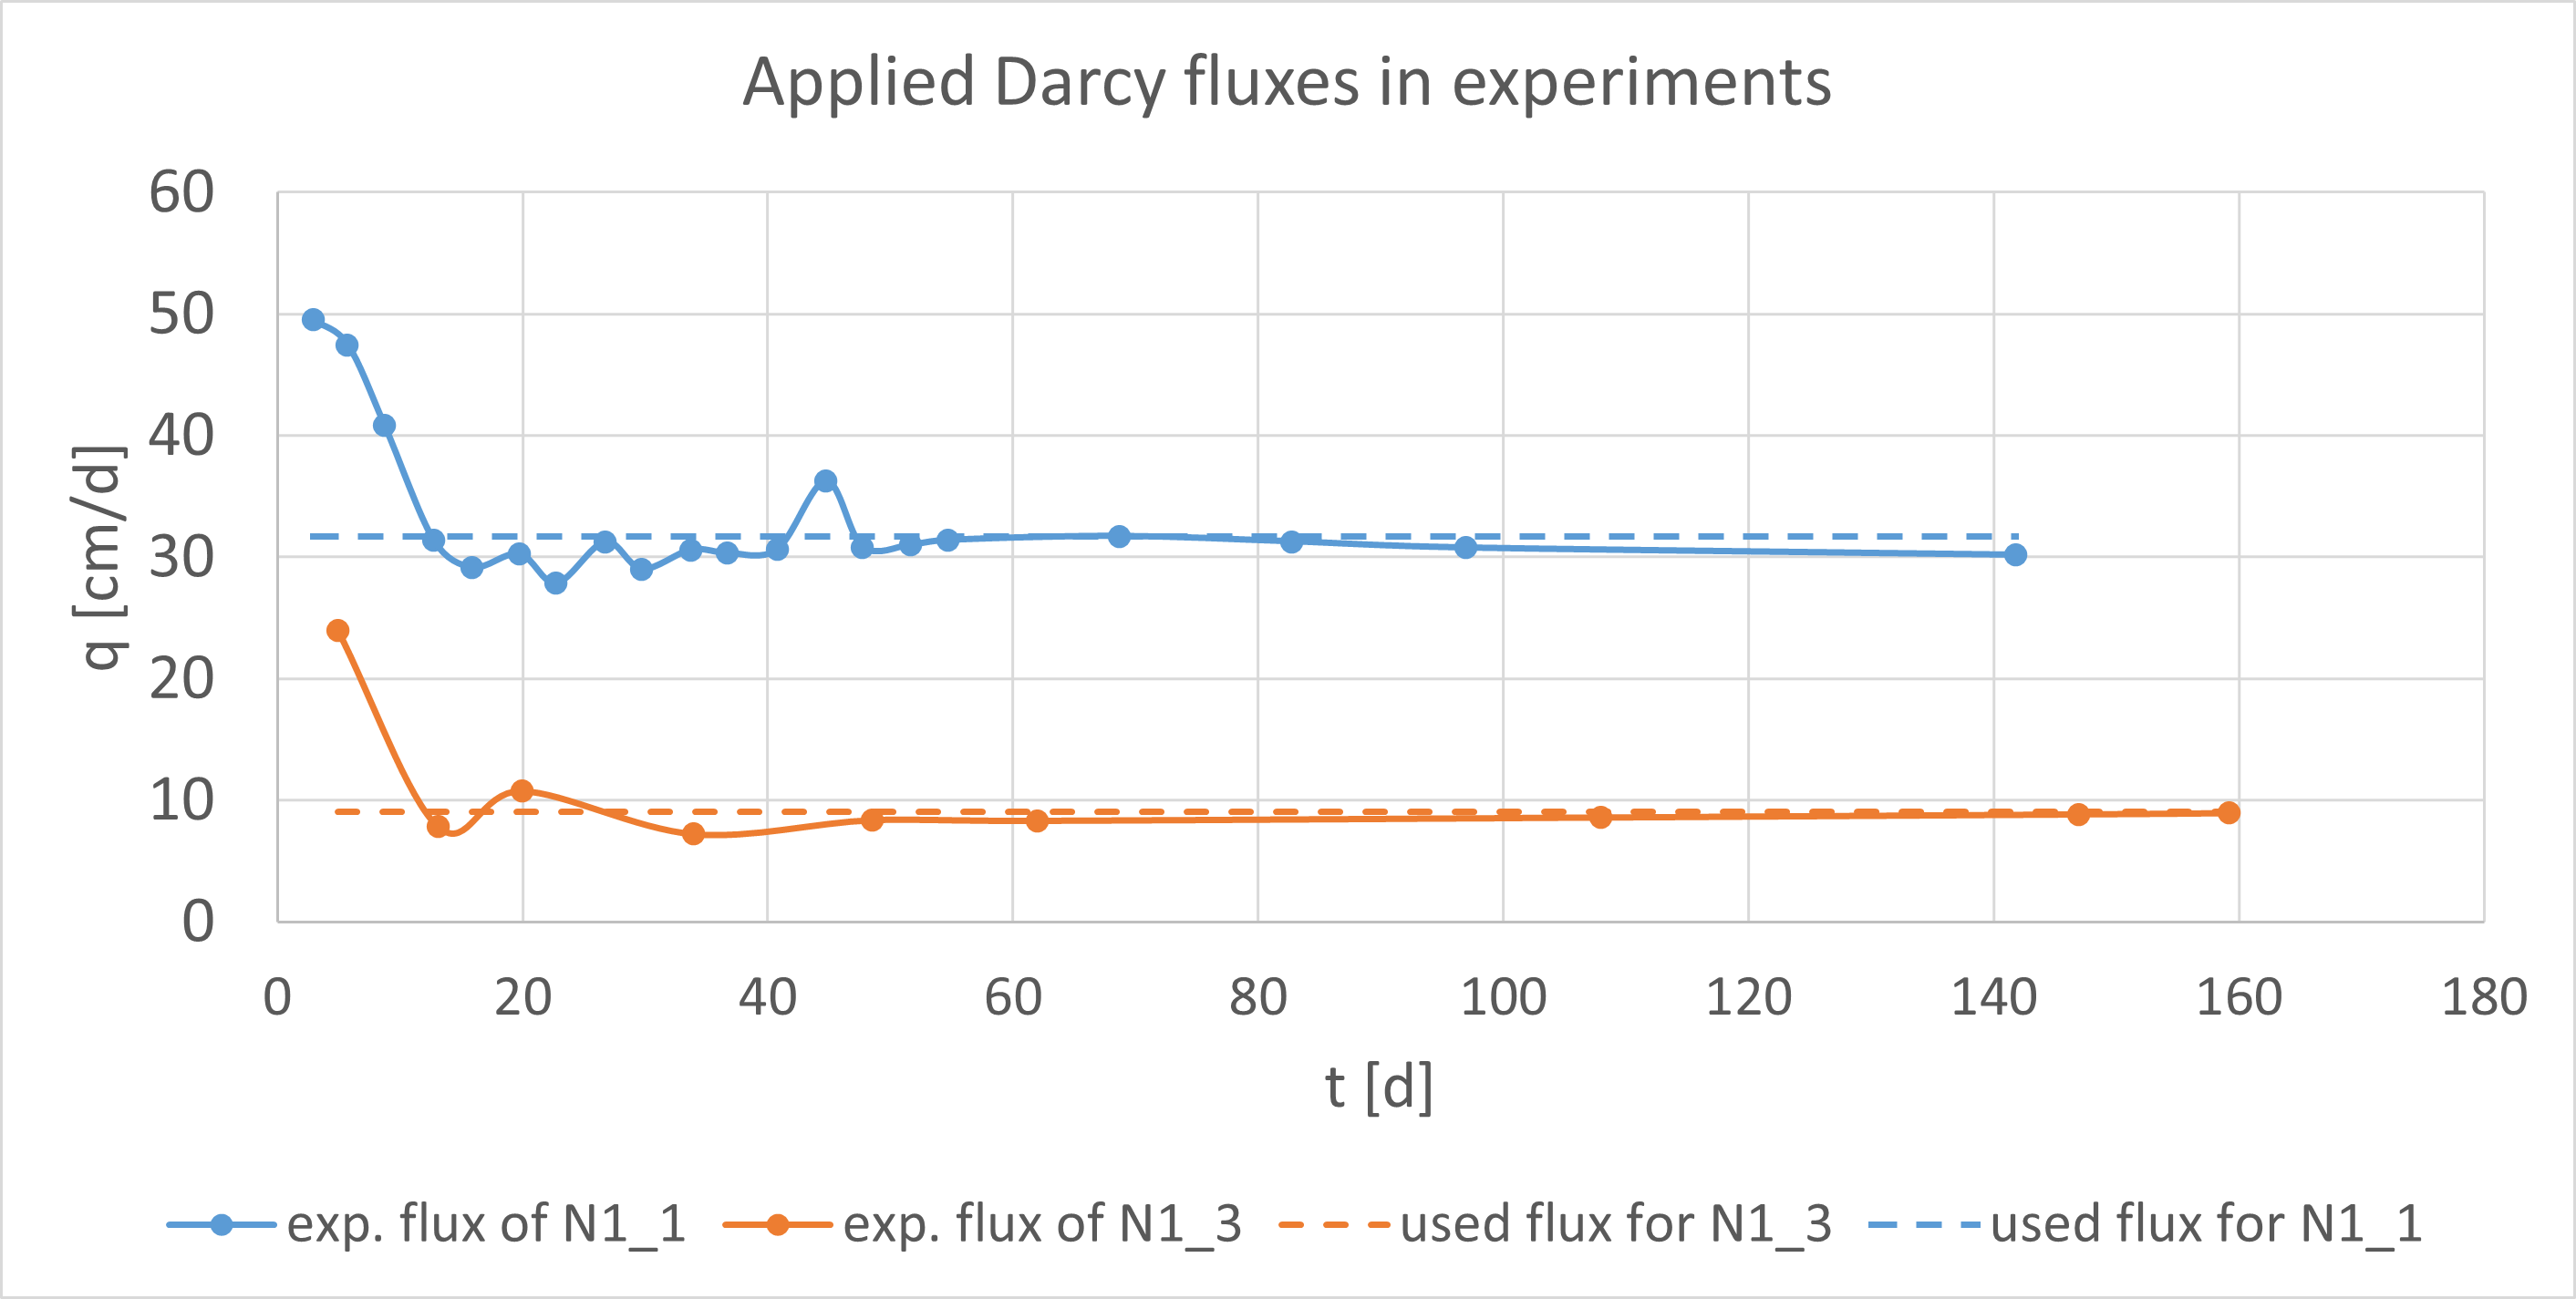
\includegraphics[scale=0.7]{images/comp_velo.png}
\caption[Different experimental Darcy fluxes]{Darcy fluxes in experiments N1\_1 and N1\_3, with used averaged Darcy fluxes for training and testing of the experimental models.}
\label{fig:different_velocities}
\end{figure}
\section{Conclusion}
In this work a FD solver for the Advection-Dispersion equation including the Two-Site model was implemented and validated with Hydrus. For 1D transport of PFOS, the solver produced plausible results for simulations without a sand layer and solutions close to the Hydrus values in contaminated soil sorrounded by two sand layers. The solution trajectories could be further used both to validate the FV procedure implemented in FINN and to provide synthetic training and test data.\\
FINN was able to reproduce the originally used model parameters of the synthetic solution to machine accuracy. Also functional relations provided good approximations for the $c$ - $s_k$ sorption isotherms after sufficient training epochs. With the loss function used for synthetic data, the BTC could only be approximated with errors for unknown sorption behaviors both in training and in \textit{in-dis-tests}.\\
Based on scarce experimental measurements at the outflow, FINN was able to learn a model for physically reasonable sorption behaviors within the contaminated soil, that provided acceptable agreement with experimental BTCs data even under other physical conditions in \textit{out-dis-tests}.\\
\\
Besides topics mentioned in the discussion sections above, in future work the physically plausible predictions about the transport and sorption behavior of PFOS could be verified by generating further experimental data at spatial coordinates inside the column. Optimally, the dissolved concentration at the beginning of the experiment should be measured, so that values and distributions of the initial dissolved concentration cannot only be estimated, as in the present work.\\
In this work only PFOS was considered. In a next step, the behaviors of other non-degradable PFASs in contaminated soil could be predicted by using corresponding experimental outflow data. Further, by extending FINN to sorption models with multiple sorption sites or incorporating reaction terms, a wide variety of chemical non-equilibrium models can be learned.\\